\documentclass[11pt,a4paper]{article}
\author{TalentSprint}
\date{}
\usepackage{verbatim}
\usepackage{fancyhdr}           % For header and footer
\usepackage{multicol}
\usepackage{colortbl}           % For coloured tables
\usepackage{setspace}           % For line height
\usepackage{seqsplit}           % Splits long words.
\usepackage{amsmath} 
\usepackage{graphicx}
\usepackage{array}
\usepackage{enumitem}
\usepackage{xcolor}
\usepackage[tikz]{bclogo}
\usepackage{textcomp}
\usepackage{listings}
\lstset{language=python,numbers=left,numberstyle=\tiny,numbersep=10pt,showstringspaces=false}

\headheight=14pt
\lhead{\nouppercase{}}
\rhead{\nouppercase{\leftmark}}

\newcommand*\lstinputpath[1]{\lstset{inputpath=#1}}
\lstinputpath{../Code/}
\graphicspath{{../Images/} {../ScreenShots/}}

\setcounter{tocdepth}{1}
\setlength\parindent{0pt}
\parskip=4pt
\newcommand{\Code}[1]{\textbf{\texttt{#1}}}

% Lengths and widths
\addtolength{\textwidth}{5cm}
\addtolength{\hoffset}{-1cm}
\setlength{\headsep}{-12pt} % Reduce space between header and content
\setlength{\headheight}{85pt} % If less, LaTeX automatically increases it
\renewcommand{\footrulewidth}{2pt} % Remove footer line
\renewcommand{\headrulewidth}{1pt} % Remove header line
\renewcommand{\seqinsert}{\ifmmode\allowbreak\else\-\fi} % Hyphens in seqsplit
% This two commands together give roughly
% the right line height in the tables
\renewcommand{\arraystretch}{1.3}
\onehalfspacing

% Commands
\newcommand{\SetRowColor}[1]{\noalign{\gdef\RowColorName{#1}}\rowcolor{\RowColorName}} % Shortcut for row colour
\newcommand{\mymulticolumn}[3]{\multicolumn{#1}{>{\columncolor{white}}#2}{#3}} % For coloured multi-cols
\newcolumntype{x}[1]{>{\raggedright}p{#1}} % New column types for ragged-right paragraph columns
\newcommand{\tn}{\tabularnewline} % Required as custom column type in use

% Font and Colours
\definecolor{HeadBackground}{HTML}{333333}
\definecolor{FootBackground}{HTML}{666666}
\definecolor{TextColor}{HTML}{333333}
\definecolor{DarkBackground}{HTML}{6B8E23} %{FD1AA8}
\definecolor{LightBackground}{HTML}{E8FED8} %D3FDC8
\definecolor{tit}{HTML}{FF6600}
\renewcommand{\familydefault}{\sfdefault}
\color{TextColor}
 \headsep = 25pt
% Header and Footer
\pagestyle{fancy}
\usepackage[headheight=110pt]{geometry}
\fancyhf{}% Clear header/footer

\fancyhead[r]{
\includegraphics[width = 4cm, height = 2cm]{TS-Logo.png}\hspace{0cm}}

%=================================TITLE=====================================
\fancyhead[l]{\Large{\bf{\textcolor{tit}{\textrm{Introduction to C}}}}}
%===========================================================================

\renewcommand{\headrulewidth}{0.4pt}% Default \headrulewidth is 0.4pt
\renewcommand{\footrulewidth}{0.4pt}% Default \footrulewidth is 0pt

\rfoot{Page \thepage}
\lfoot{COPYRIGHT \textcopyright TALENTSPRINT, 2015. ALL RIGHTS RESERVED.}




\begin{document}


%\chapter{Introduction to C}

\section*{History}

C is a general purpose programming language. It was developed by Dennis Ritchie at AT\&T  Bell Laboratories in the year 1972. It was developed along with the Unix Operating System. C was extensively used in its development. It was first implemented on the Digital Equipment Corporation PDP-11 computer.

C is an outgrowth of an earlier language B which was itself based on BCPL (Basic Combined Programming Language). 

The Unix operating system and almost all Unix applications are written in the C language. C has now become a widely used professional language for the following reasons:

\begin{itemize}
\item It produces efficient programs.
\item It can handle low-level activities.
\item It can be compiled on a variety of computers.
\end{itemize}

The C language was formalized in 1988 by the American National Standard Institute (ANSI). The latest standard is referred to as c11 and stands for the ISO/IEC 9899:2011. Since that is relatively new, the most often used standard is likely to be \textbf{\texttt{c99}}. We will be using c99 in this course.

\section*{C usage}
C was initially used for system development work. It is suitable for this, as it produces code that runs nearly as fast as assembly. 

Some such uses of C are:
%\begin{comment}
\begin{itemize}
\item  Operating Systems: Unix, Linux
\item  Language Compilers: CCS C Compiler, Dev-C++, Digital Mars
\item  Assemblers
\item  Text Editors: vi Text Editor
\item  Network Drivers
\item  Language Interpreters: Python
\end{itemize}
%\end{comment}

\section*{Sample Program}
Now let us write our first C program. It will display \emph{Hello World!} on the screen. To create, compile and execute the program, follow these steps:

\begin{enumerate}
\item Open the file using \textbf{vim Program-01-1.c} and type the following lines in that file and save.

\lstinputlisting{Program-01-1.c}

\item Now type the below command in terminal to compile the program.
\begin{verbatim}
     c99 Program-01-1.c 
\end{verbatim}

\item Now type the below command in terminal to execute the program. 
\begin{verbatim}
     ./a.out
\end{verbatim}

Whenever the source program is modified, the entire process of compiling and executing the program should be repeated.
\begin{bclogo}[couleur=blue!5, arrondi=0.3, logo=\bctrombone]{Note}
In Unix/Linux, by default the C compiler will produce an executable file called \textbf{\texttt{a.out}}. We can either give another name while compiling or rename the executable file after compiling. For example, \texttt{c99 Program-01-1.c -o hello} will produce an executable named \texttt{hello}.
\end{bclogo}
\end{enumerate}

\begin{figure}[ht]
\begin{center}
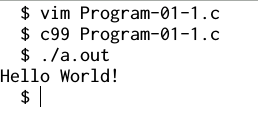
\includegraphics{Output-01-1.png}
\caption{Output}
\label{output-01-1}
\end{center}
\end{figure}

\section*{Toolset}

Three things are necessary for creating C programs:

\begin{description} 
\item[Text Editor]  A text editor is a program used for writing and editing plain text. It differs from a word processor in that it does not do formatting such as typefaces, fonts, margins and italics.  C programs can be written using any of the many text editors that are available for Linux such as \textbf{\texttt{vim, gedit, nano, emacs}}.
\item [Compiler] A compiler is a specialized program that converts source code into machine language (also called object code or machine code) so that it can be executed by a CPU (central processing unit).
\item [C Standard Library] The C standard library is a collection of header files and library routines used to implement common operations, such as input/output and string handling, so nearly all C programs rely on the standard library functions.
\end{description} 

There are four phases involved in compilation process:
\begin{description} 
\item [Preprocessing] The C preprocessor --in Unix/Linux it is a program called \textbf{\texttt{cpp}}-- is a macro processor that is used automatically by the C compiler to transform your program before compilation. It is called a macro processor because it allows you to define macros, which are brief abbreviations for longer constructs.
\item [Compilation] Source code for C programs are written as ASCII text. They must be \emph{compiled} and \emph{linked} to produce \emph{executable} programs. The executable files are what you actually run. The compilation of code involves several steps:
  \begin{itemize}
  \item parsing of the statements for syntax
  \item translation of the statements into assembly language instructions
  \item setting up the addresses of all variables and functions
  \end{itemize}
\item [Assembly] C is a high-level compiled language. The process of compilation is very complex, but the basic operation resembles that of assembly, with one exception -- each line of the program can produce one or more machine code instrcutions. The assembler takes as its source code an assembly language program, this is also a file of ASCII characters, it used this to produce machine code.
\item [Linking] When a programmer needs a library, he specifies the library to the compiler/assembler. The compiler/assembler then doesn't try to find the address of the procedure, but instead leaves this to the linker. It provides the name of the appropriate libary file to the linker. The linker then processes the object code which was generated. It searches the known sets of library files and connects up the references to the library code with the actual code. 
\end{description} 

\begin{figure}[ht]
\begin{center}
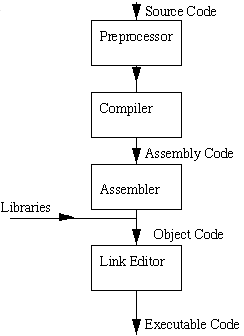
\includegraphics[scale=0.5]{CompilingStages.png}
\end{center}
\caption{Compilation Phases}
\label{ccStages}
\end{figure}

\section*{Building blocks of C Program}
In order to understand the functioning a program, we need to understand the role of the following four elements: Preprocessor commands, Functions, Variables and Comments. It should be noted that this perspective is in no way intended as describing the structure of a program. 
\begin{description}
\item [Preprocessor Commands] All preprocessor lines begin with `\#'. These commands tells the compiler to do preprocessing before doing actual compilation. For example, \texttt{\#include \textless stdio.h\textgreater} is a preprocessor command which tells a C compiler to include \texttt{\textless stdio.h\textgreater} file before going to actual compilation. The C Preprocessor is not part of the compiler, but it is a separate program called internally by the compiler. 
\item [Functions] Functions are main building blocks of any C Program. Every C Program will have one or more functions and there is one mandatory function which is called \textbf{\texttt{main()}} function. The C program execution starts from \emph{main()} function. We will discuss functions in detail later.
\item [Variables] Variables are simply names used to refer to some location in memory, a location that holds a value with which we are working. Within the C programming language, when managing and working with variables, it is important to know the type of variables and the size (memory required) of these types. 
\item [Statements] Statements can be expressions, assignments, function calls, or control flow statements which make up C program. Expressions combine variables and constants to create new values.
\item [Block] A block is a lexical grouping of statements and can be thought of as \emph{one} logical statement. A block in C is delimited by braces: \{ and \}.
\item [Comments] Comments are used to give additional useful information inside a program. you can place comments in your code that are not executed as part of the program. A block comment is used when the comment will span several lines. A block comment starts with /* symbol and ends with */ and can be anywhere in your program. The line comment uses two slashes ($/$$/$), generally used for short comments.
\end{description}

\section*{Header Files}
All header files should be included explicitly before \textbf{\texttt{main()}} function. They have the extension \emph{.h}.

A header file contains declarations of different predefined functions, which are used in the program. A header file may also contain macros. This allows programmers to separate functions of a program into reusable chunks. 

The prototypes of library functions are gathered together into various categories and stored in header files. For example, all prototypes of standard input/output functions are stored in header file \emph{`stdio.h'}, while the mathematical functions such as sine are in \emph{`math.h'}. 

The header files can be declared in two ways.

\begin{verbatim} 
     #include "Aheader"
     #include <Bheader>
\end{verbatim}

Now Aheader will be looked for in the current directory, while Bheader will be looked for in the standard header file locations: most probably `/usr/include' in Unix systems.

\subsection*{Standard Headers}
Following are the most commonly used header files, presented in alphabetical order.
\begin{itemize}
\item assert.h
\item ctype.h
\item graphics.h	
\item math.h
\item process.h
\item stdio.h
\item stdlib.h
\item string.h
\item time.h
\end{itemize}

\section*{Naming Rules in C}
There are rules for choosing the character sequence to be used for identifiers which denote variables, types and functions. Such identifiers must begin with an alphabet or underscore, and may be followed by any combination of alphabets, underscores, or the digits 0-9.

Please note that C is case sensitive; uppercase and lowercase alphabets are treated as distinct.

You should ensure that you use meaningful names for your identifiers. Please note meaningful \emph{does not} necessarily mean long. The goal is to make the program easier to read and be self-documenting. Compare the two segments:

\begin{verbatim}      
   distance = speed * time;
   s = v * t;    
\end{verbatim}

Most users adopt the convention that variable names are all lower case, while names for constants are all upper case.

\section*{Keywords}
Keywords are reserved identifiers that have strict meaning to the C compiler and hence cannot be used as identifiers in your program.

\texttt{
\begin{table}[h]
\centering
\begin{tabular}{l l l l}\\
auto  & break & case & char\\
const & continue & default & do\\
double & else & enum & extern\\
float & for & goto & if\\
int & long & register & return\\
short & signed & sizeof & static\\
struct & switch & typedef & union\\
unsigned & void & volatile & while\\ 
\end{tabular}
\caption{List of C keywords}
\end{table}
}

\section*{Additional notes}

\begin{bclogo}[couleur=blue!5, arrondi=0.3, logo=\bctrombone]{Note}
C is a procedural language. A procedural language is a programming language that uses procedures (aka subroutines or functions) as the unit of execution and modularisation. A procedure contains a self-contained set of statements that execute to produce a desirable output.
\end{bclogo}
\end{document}